\chapter{sviluppo applicazioni web}


In questo capitolo si fornisce un survey delle patologie dell'ingegnere...

%
% Commento: questa � la prima sezione
%
\section{storia web}

\index{Titolo per indice della sezione}

Qui inseriamo un riferimento \cite{a}.

\subsection{Titolo sottosezione}

%\begin{figure}[tp]
%    {\begin{center}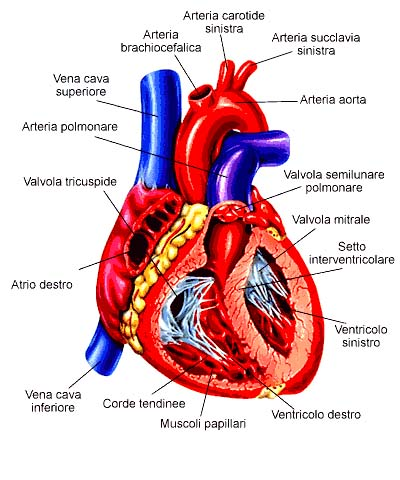
\includegraphics[width=8cm]{figure/cuore_aperto.jpg}\end{center}}
%\caption{Il cuore  \label{cuore}}
%\end{figure}

Come si vede in figura \ref{cuore}...

Attenzione agli accenti:   \`{e}, perch\'{e}

Riferimento ad un sito \cite{mysite}...

\subsection{Seconda sottosezione}

bla bla

